\documentclass{article}

\usepackage{graphicx}
\usepackage{hyperref}
\usepackage[a4paper, margin=1in]{geometry}
\usepackage{breakcites}
\usepackage{subcaption}
\usepackage{float}
\usepackage{textcomp}
\usepackage{amsmath}
\usepackage{textgreek}
\usepackage{authblk}
\usepackage{rotating}
\usepackage{booktabs}
\usepackage{longtable}
\usepackage{pdflscape}
\usepackage{subcaption}
\usepackage{lineno}
\usepackage{fancyhdr}
\usepackage[
  style=numeric,
  citestyle=numeric-comp,
  backend=biber,
  doi=true,
  natbib=true,
  sorting=none
]{biblatex}

\pagestyle{fancy}
\fancyhf{}
\lfoot{Supplemental Materials for \textit{Fine-scale Twitter Big Data Reveals Neighborhood Inequalities in Mental Health Effects of High Temperatures}}
\rfoot{\thepage}

\renewcommand{\footrulewidth}{0.4pt}
\renewcommand{\headrulewidth}{0pt}


\addbibresource{TextDataClimateShocks.bib}

\begin{document}
\begin{center}
\section*{Supplemental Materials for \textit{Fine-scale Twitter Big Data Reveals Neighborhood Inequalities in Mental Health Effects of High Temperatures}}
\end{center}

\setcounter{table}{0}
\setcounter{figure}{0}
\setcounter{section}{0}
\renewcommand{\thetable}{S\arabic{table}}
\renewcommand{\thefigure}{S\arabic{figure}}
\renewcommand{\thesection}{S\arabic{section}}

\section{Alternative Sentiment Algorithms}

\subsection{Hedonometer}

In addition to the Valence Aware Dictionary for sentiment Reasoning (VADER) sentiment analysis method \cite{gilbert_vader_2014}, we also used the hedonometer method \cite{Dodds2011Dec}.  This sentiment metric yielded very similar findings to those presented in the main paper with the VADER method.

The Hedonometer \cite{dodds_temporal_2011} is a corpus-based technique to get sentiment score from multi-lingual texts. The core steps are (1) building human evaluations of the happiness of a set of individual words, and (2)using a naive algorithm for scaling up from individual words to texts. For the English corpus, Dodds and others \cite{dodds_temporal_2011} collect 10,222 unique words and used crowd-sourcing platform Amazon Mechanical Turk to get human evaluation of happiness degree for each word in an integer scale from 1 to 9, representing a sad to happy spectrum. Score 5 represents neutral words. Each word will be calculated average score and then the word and happiness score are compiled into a dataset (labMT 1.0). Some illustrative example of words are: 

\[h_{avg} (\text{laughter}) = 8.50 \]
\[h_{avg} (\text{the}) = 4.98\]
\[h_{avg} (\text{hate}) = 2.34\]

The sentiment score for single text will be the mean happiness score for all words in the text.

\begin{figure}[H]
  \centering
  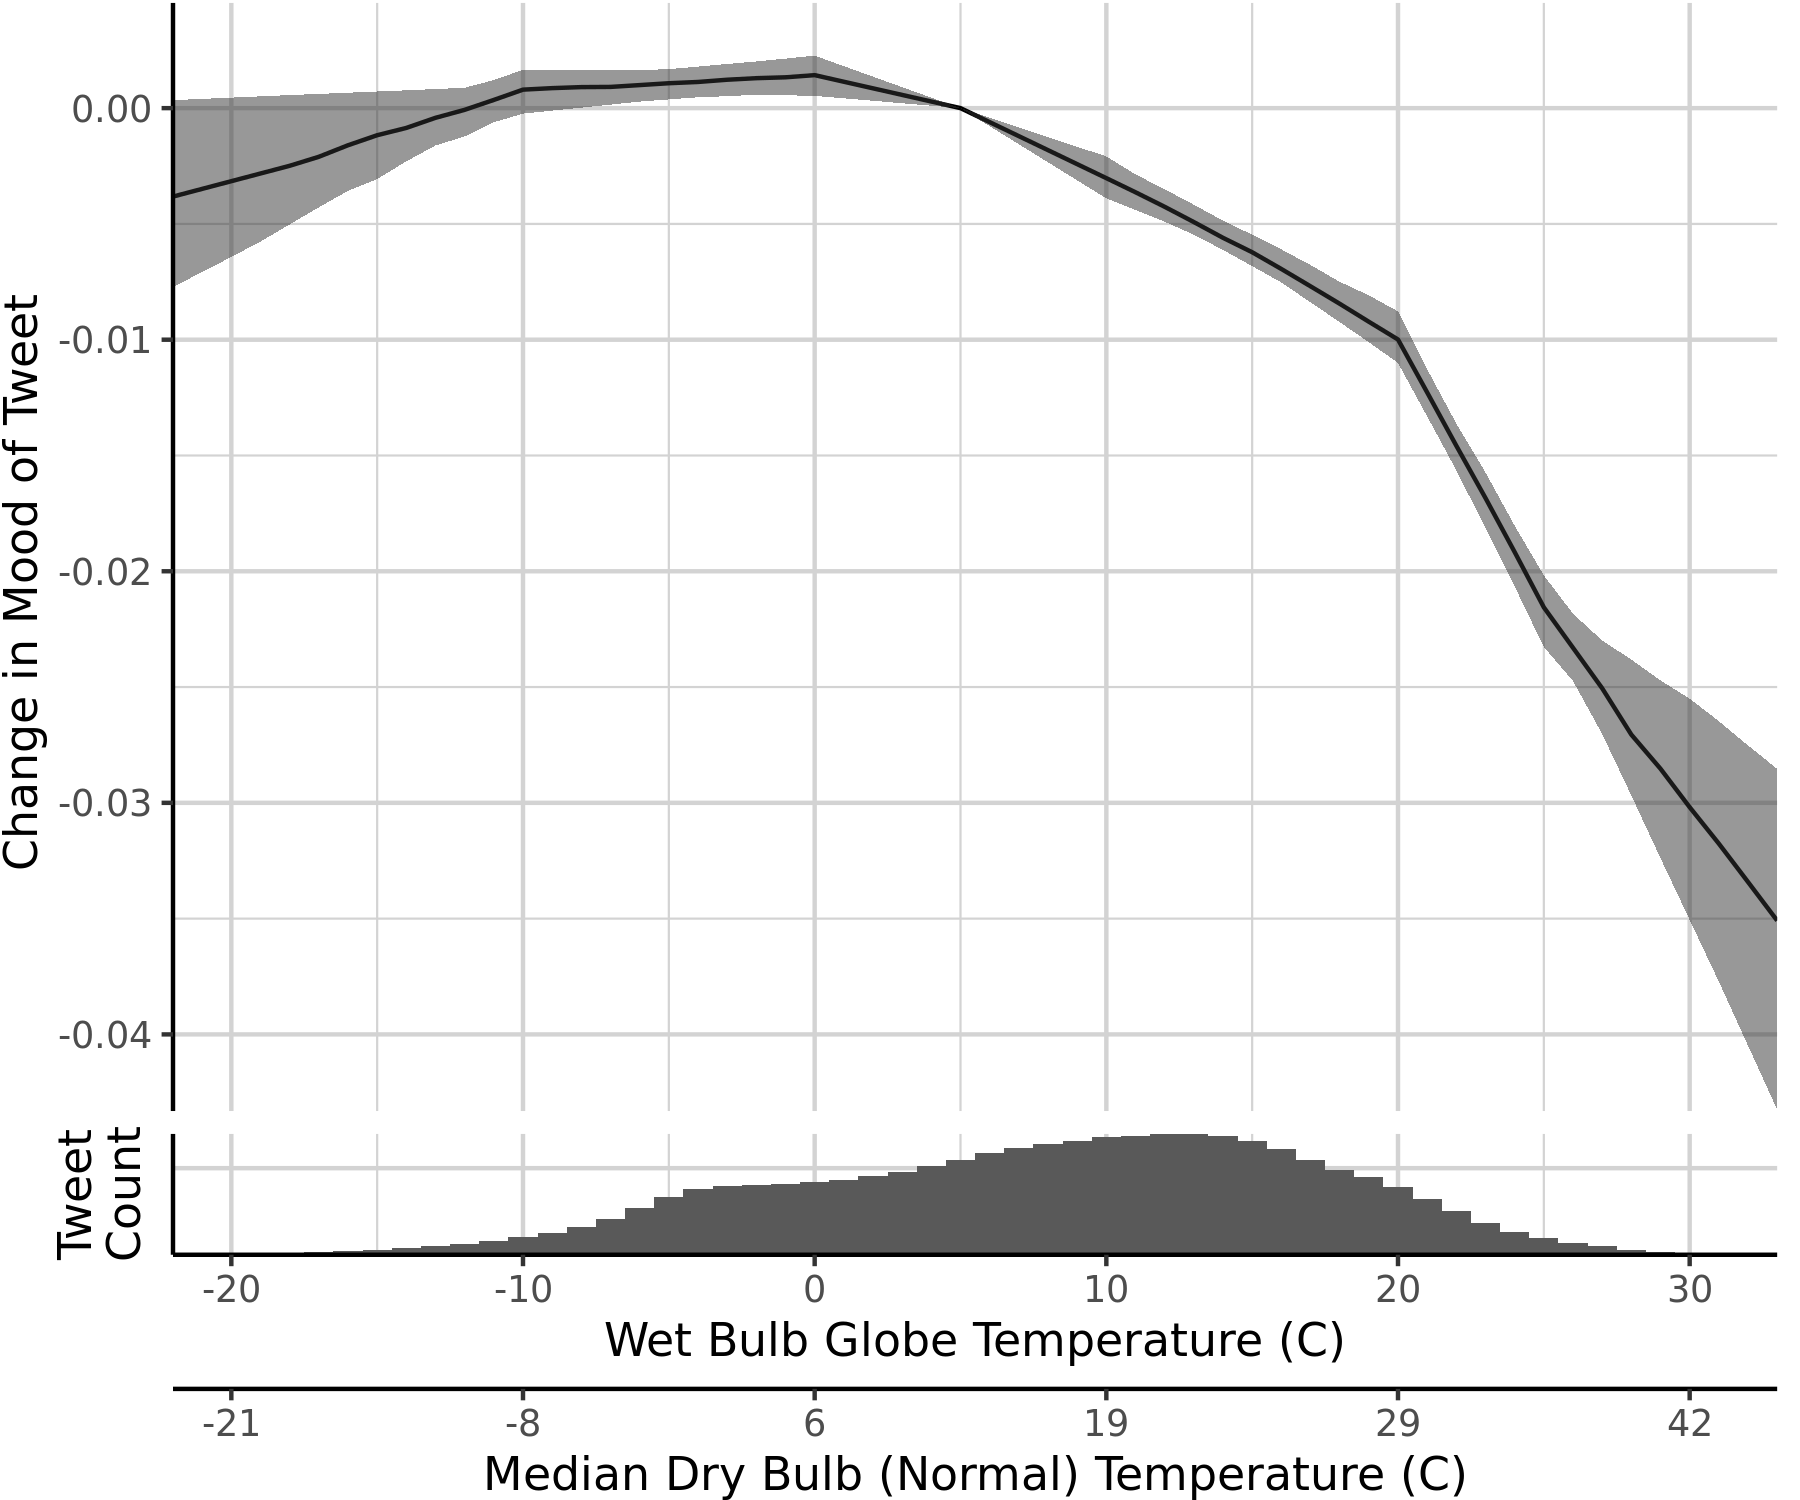
\includegraphics[width=0.6\linewidth]{../res/hedono-wbgt.png}
  \caption{Effects of temperature on sentiment, measured with the hedonometer method.}
\end{figure}

\begin{figure}[H]
  \centering
  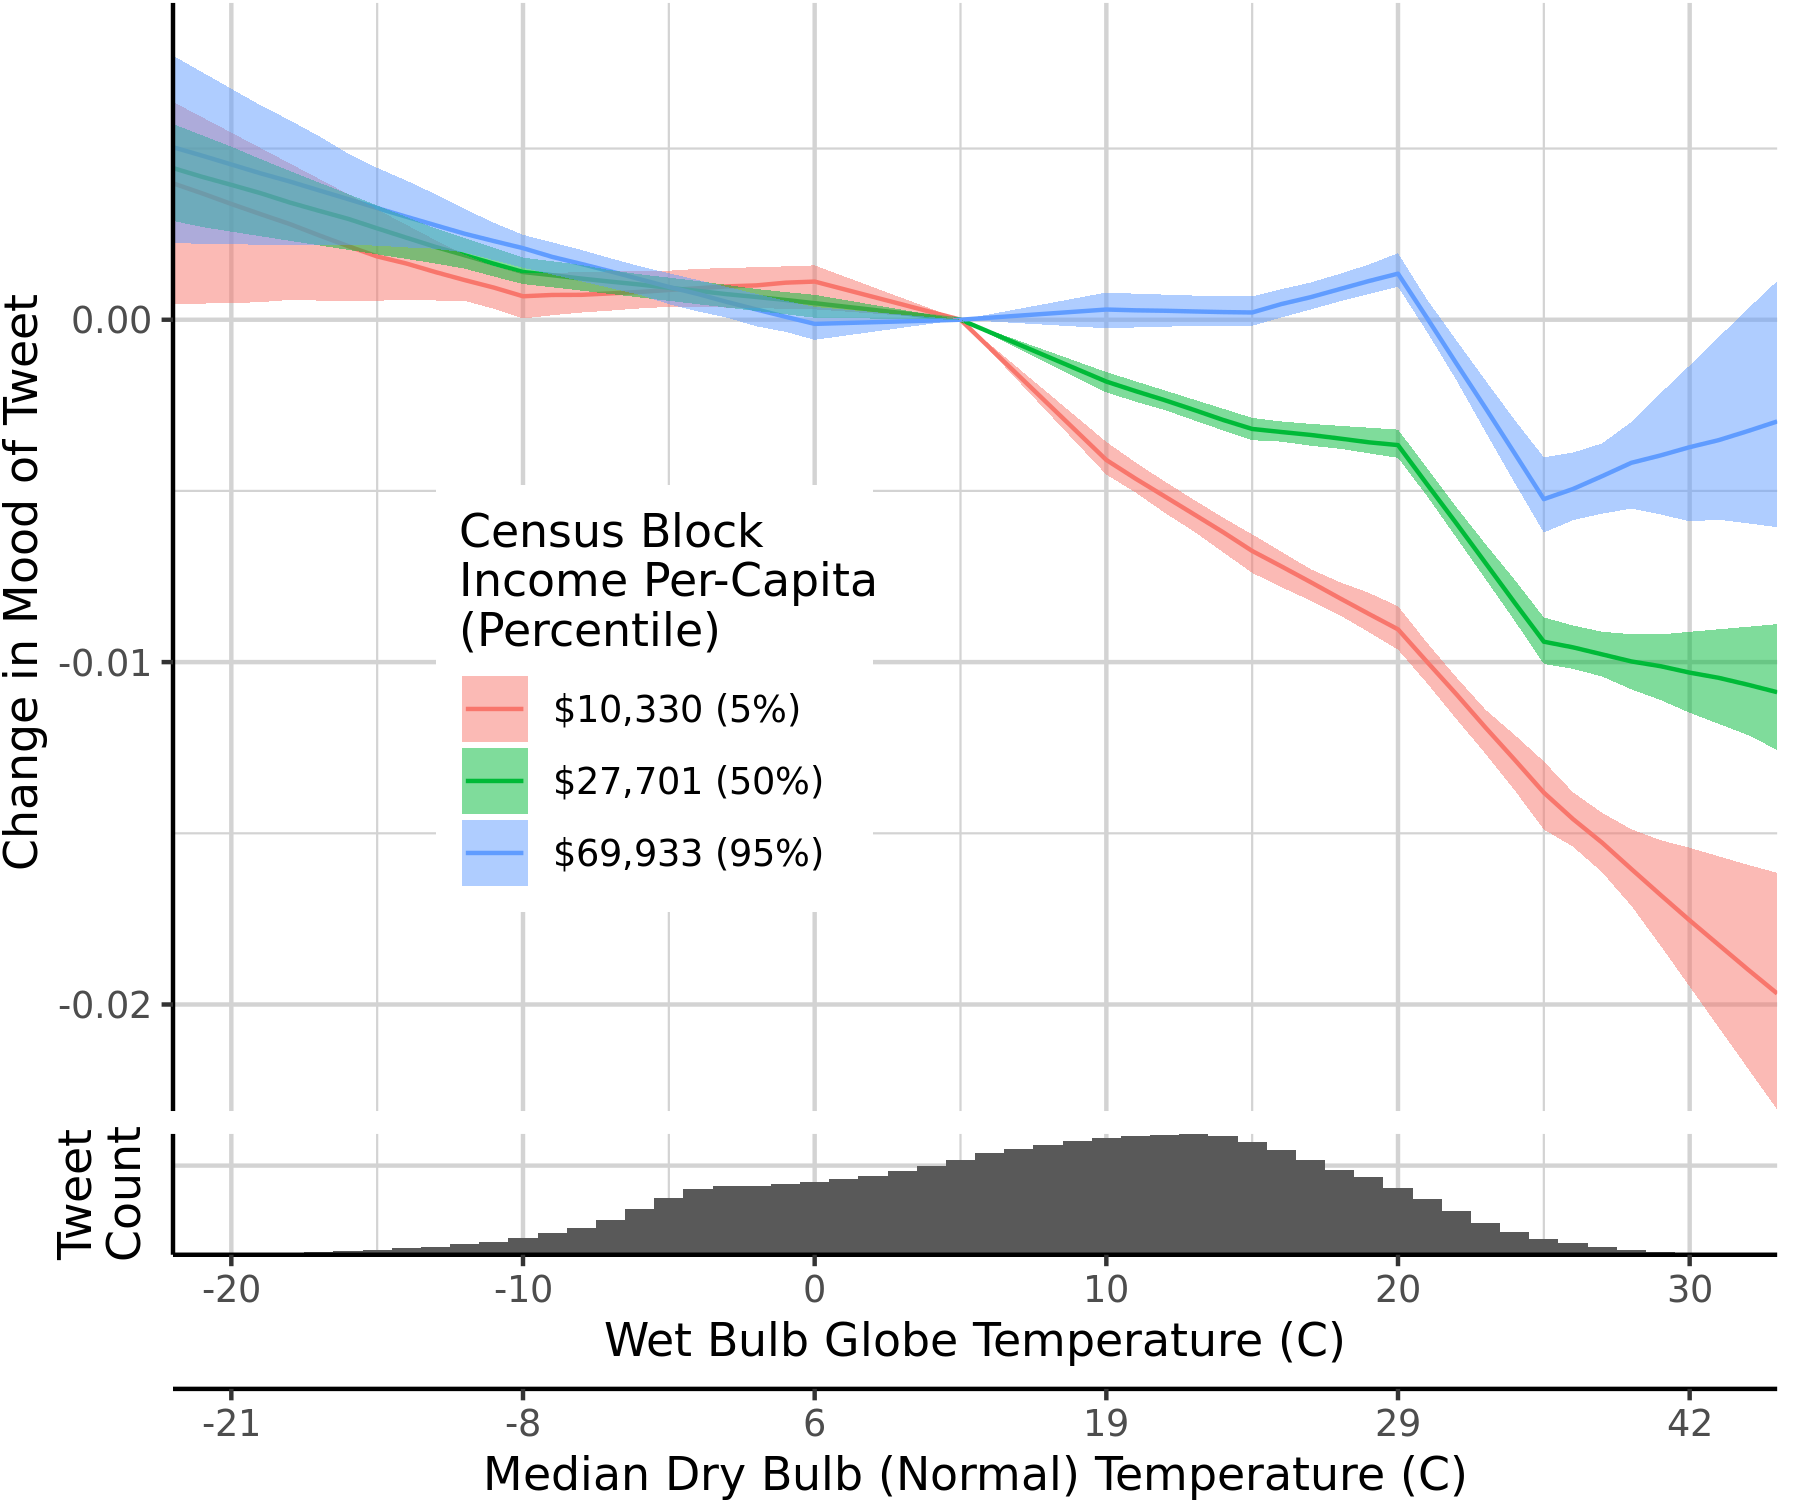
\includegraphics[width=0.6\linewidth]{../res/hedono-wbgt-income.png}
  \caption{Effects of temperature on sentiment and moderated by income, measured with the hedonometer method.}
\end{figure}

\begin{figure}[H]
  \centering
  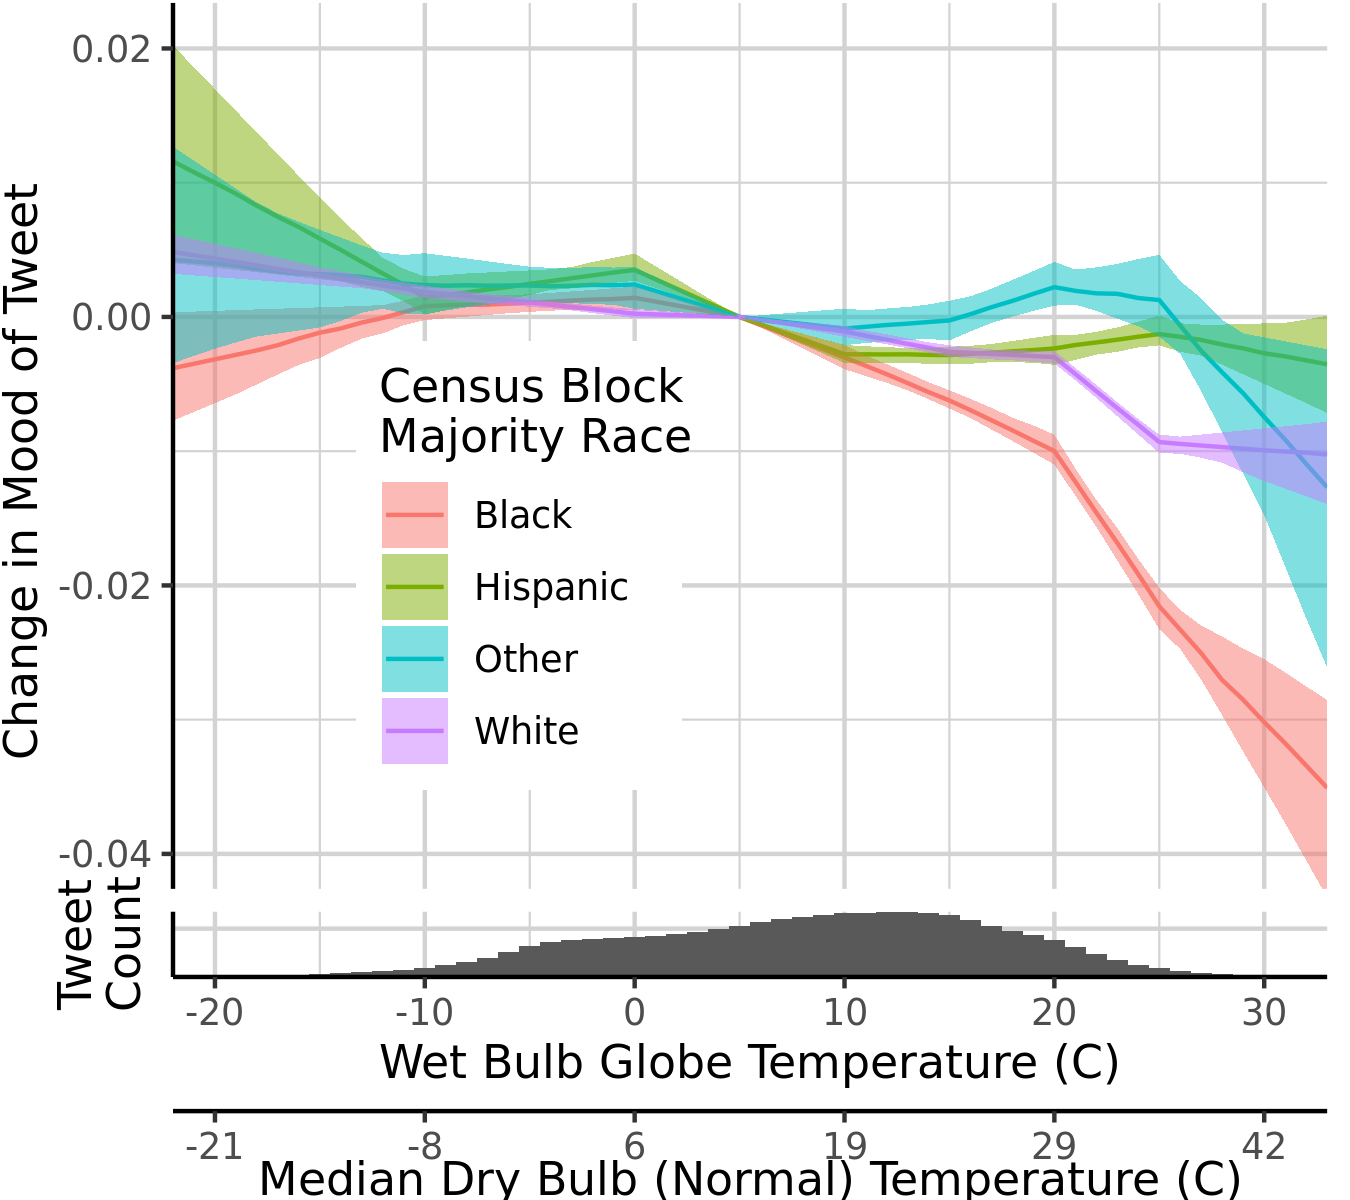
\includegraphics[width=0.6\linewidth]{../res/hedono-wbgt-race_q.png}
  \caption{Effects of temperature on sentiment and moderated by race, measured with the hedonometer method.}
\end{figure}

\subsection{AFINN}

\section{Alternative Interaction Variables}
For our main analysis, we treated income as a continuous (log-transformed) variable and race as a categorical variable.  We ran similar analyses with income as a categorical variable and race as a continuous variable (the percent of a census block's population that was non-white/minority).

\begin{figure}[H]
  \centering
  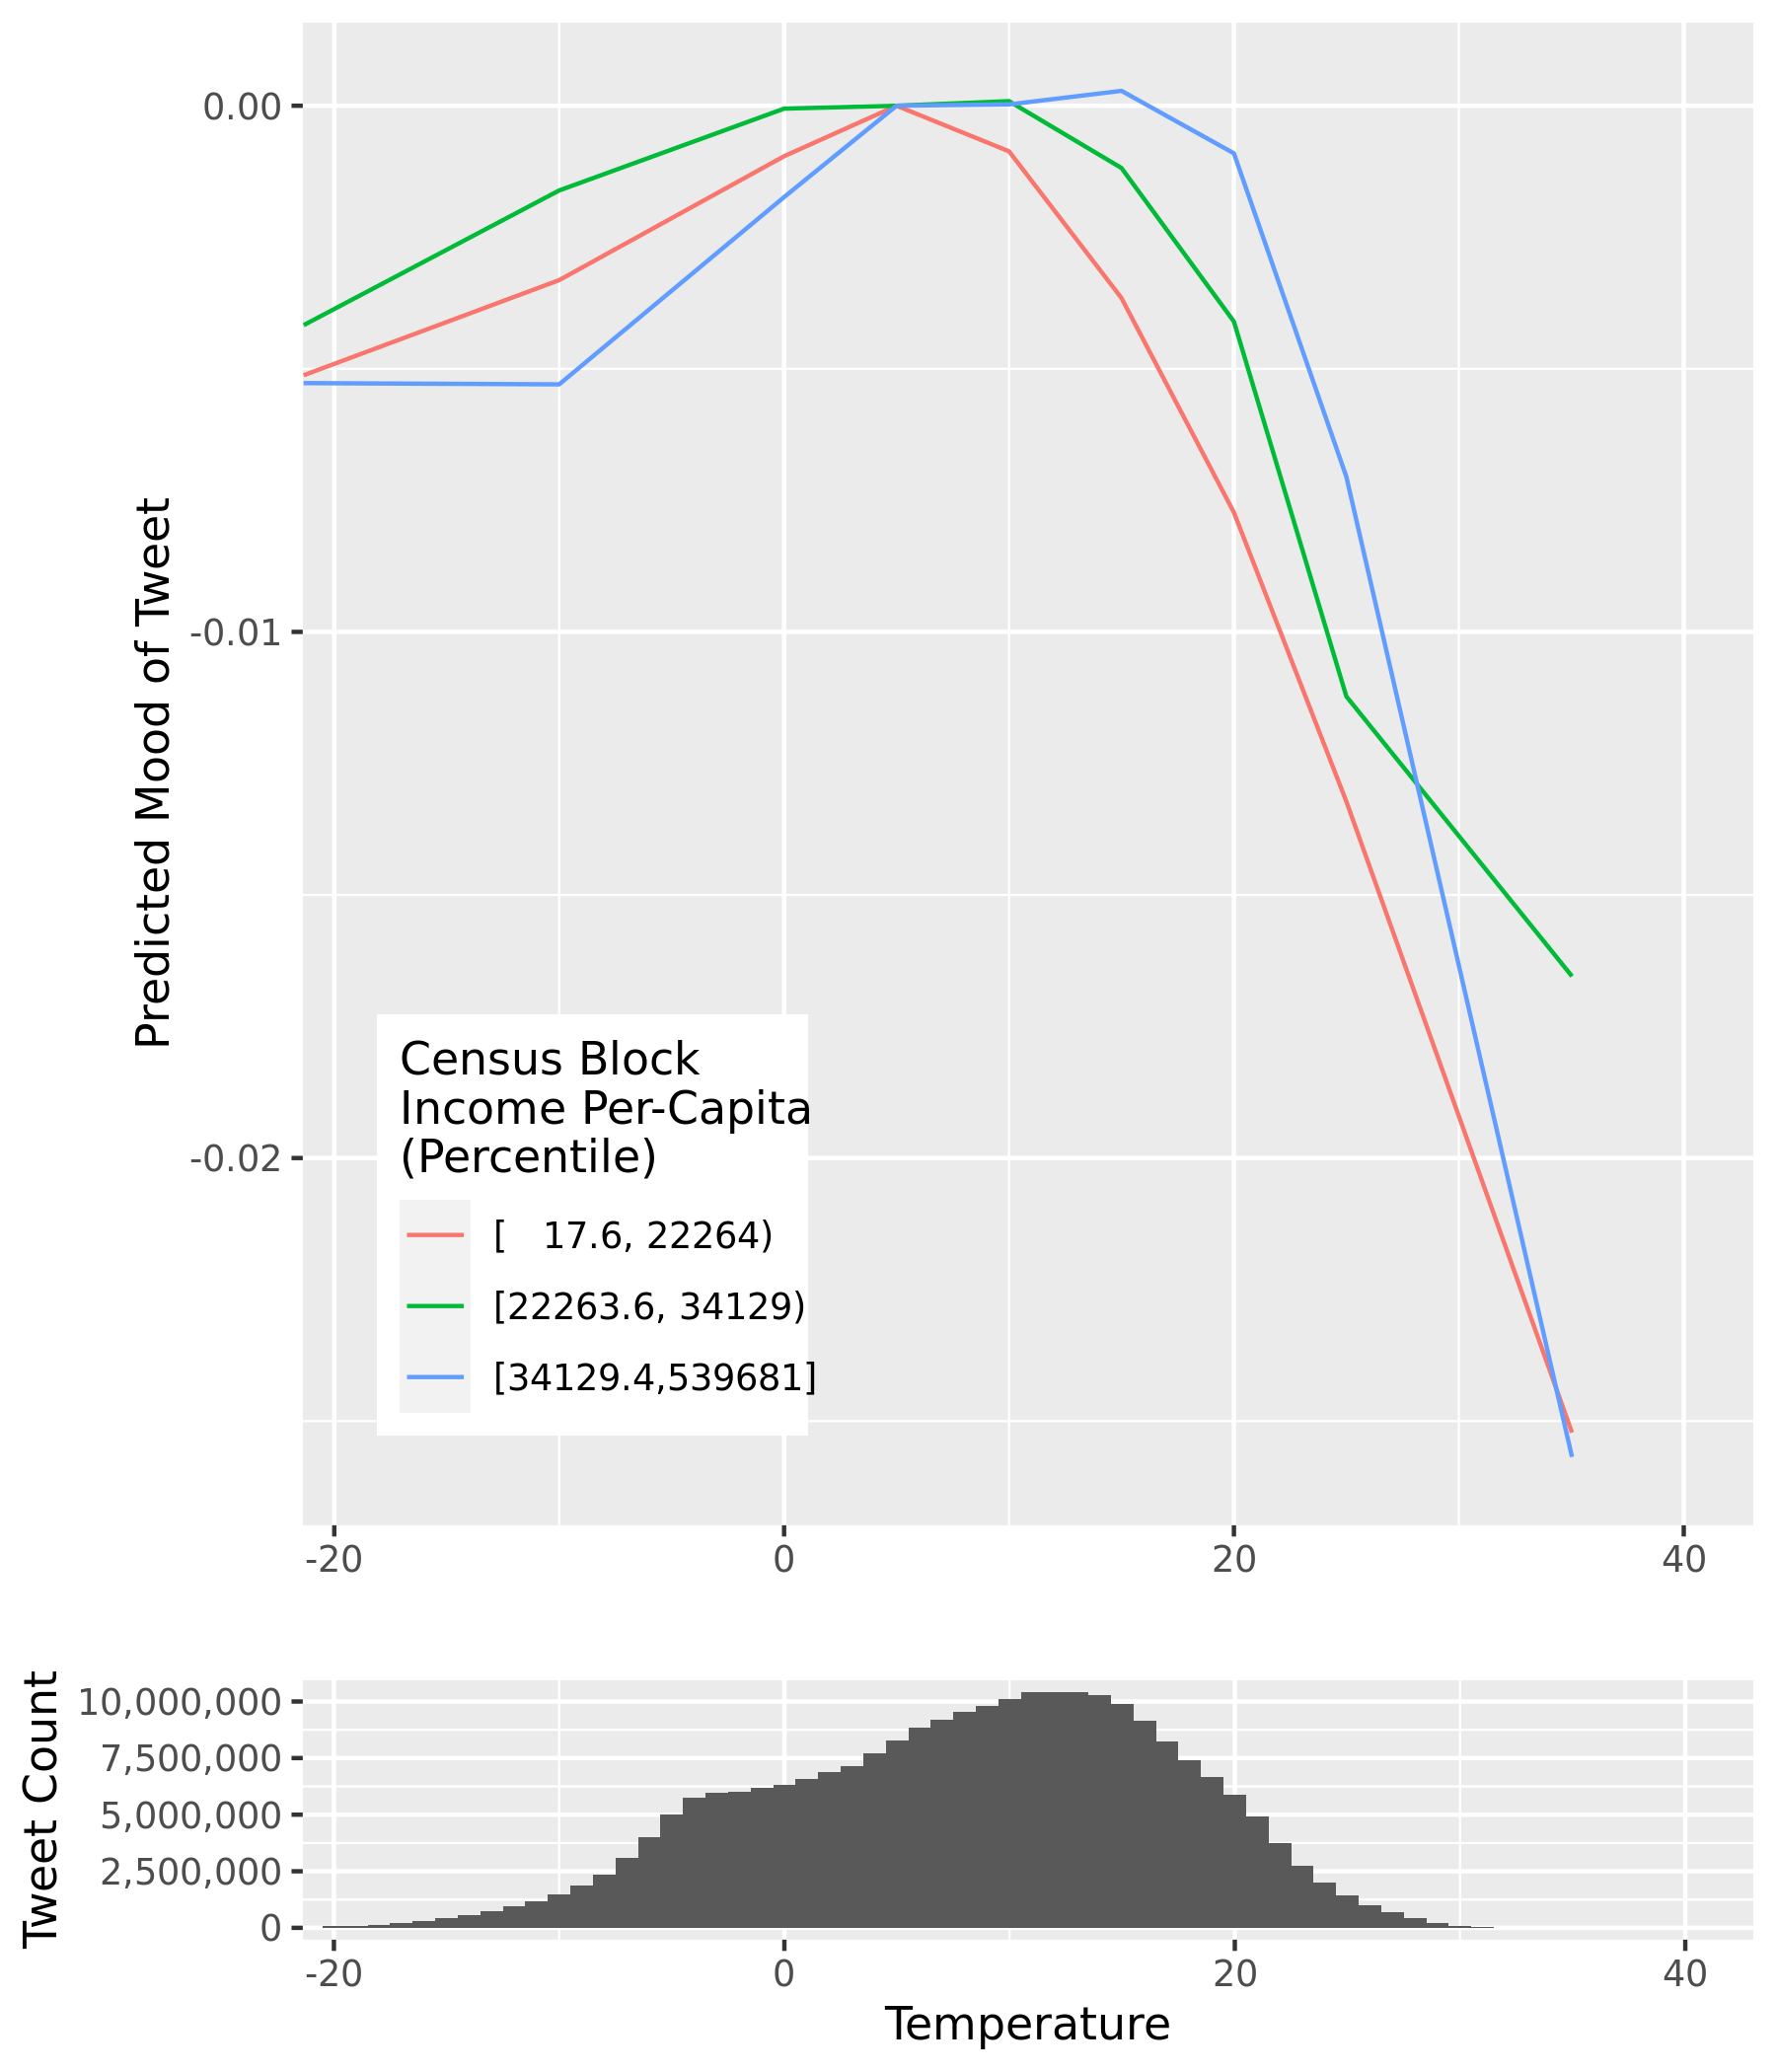
\includegraphics[width=0.6\linewidth]{../res/wbgt-income_q.png}
  \caption{Effect of temperature on sentiment and moderated by income, with income as a categorical variable.}
\end{figure}

\begin{figure}[H]
  \centering
  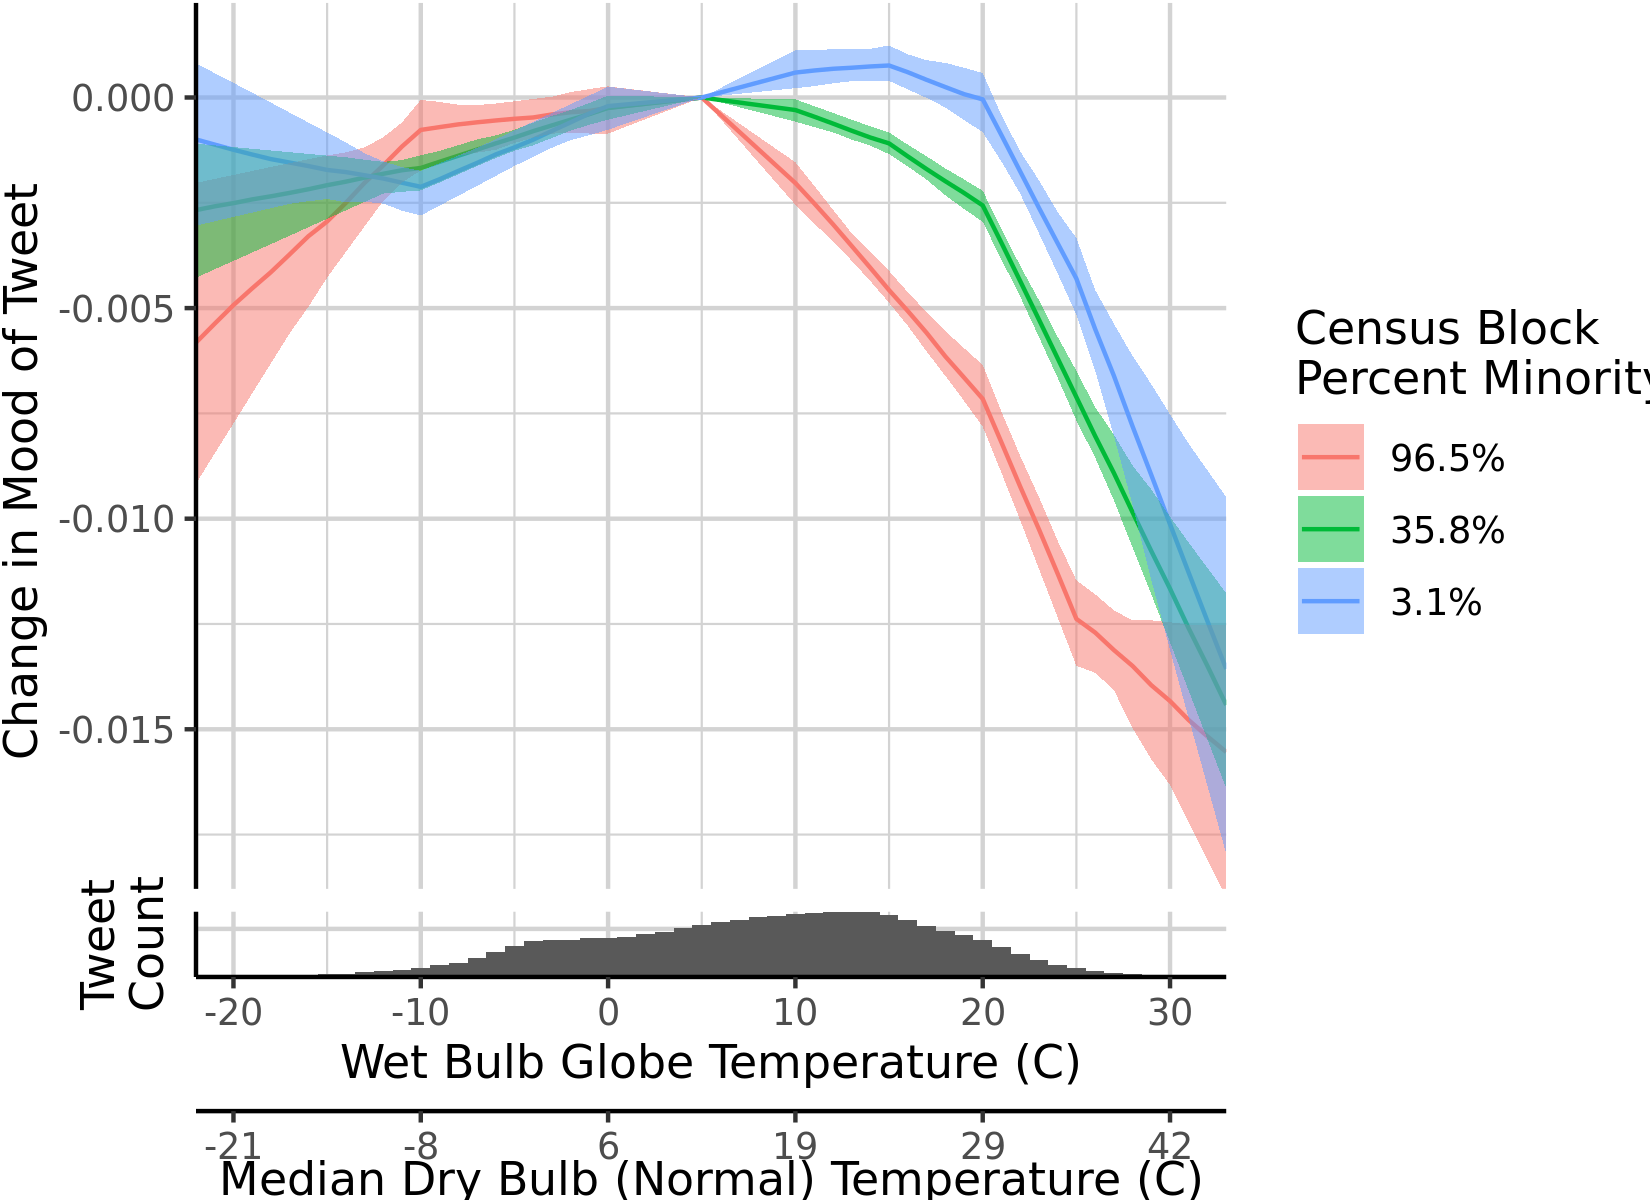
\includegraphics[width=0.6\linewidth]{../res/wbgt-race.png}
  \caption{Effect of temperature on sentiment and moderated by race, with race as a continuous variable.}
\end{figure}

\section{Effects of Precipitation and Sunshine}
While our main variable of interest was temperature as measured by Wet Bulb Globe Temperature, we also interacted our variables of interest with a binary variable for whether it was raining or not, as well as a continous variable for the amount of shortwave radiation in ($W/m^2$), or sunshine.

\begin{figure}[H]
  \centering
  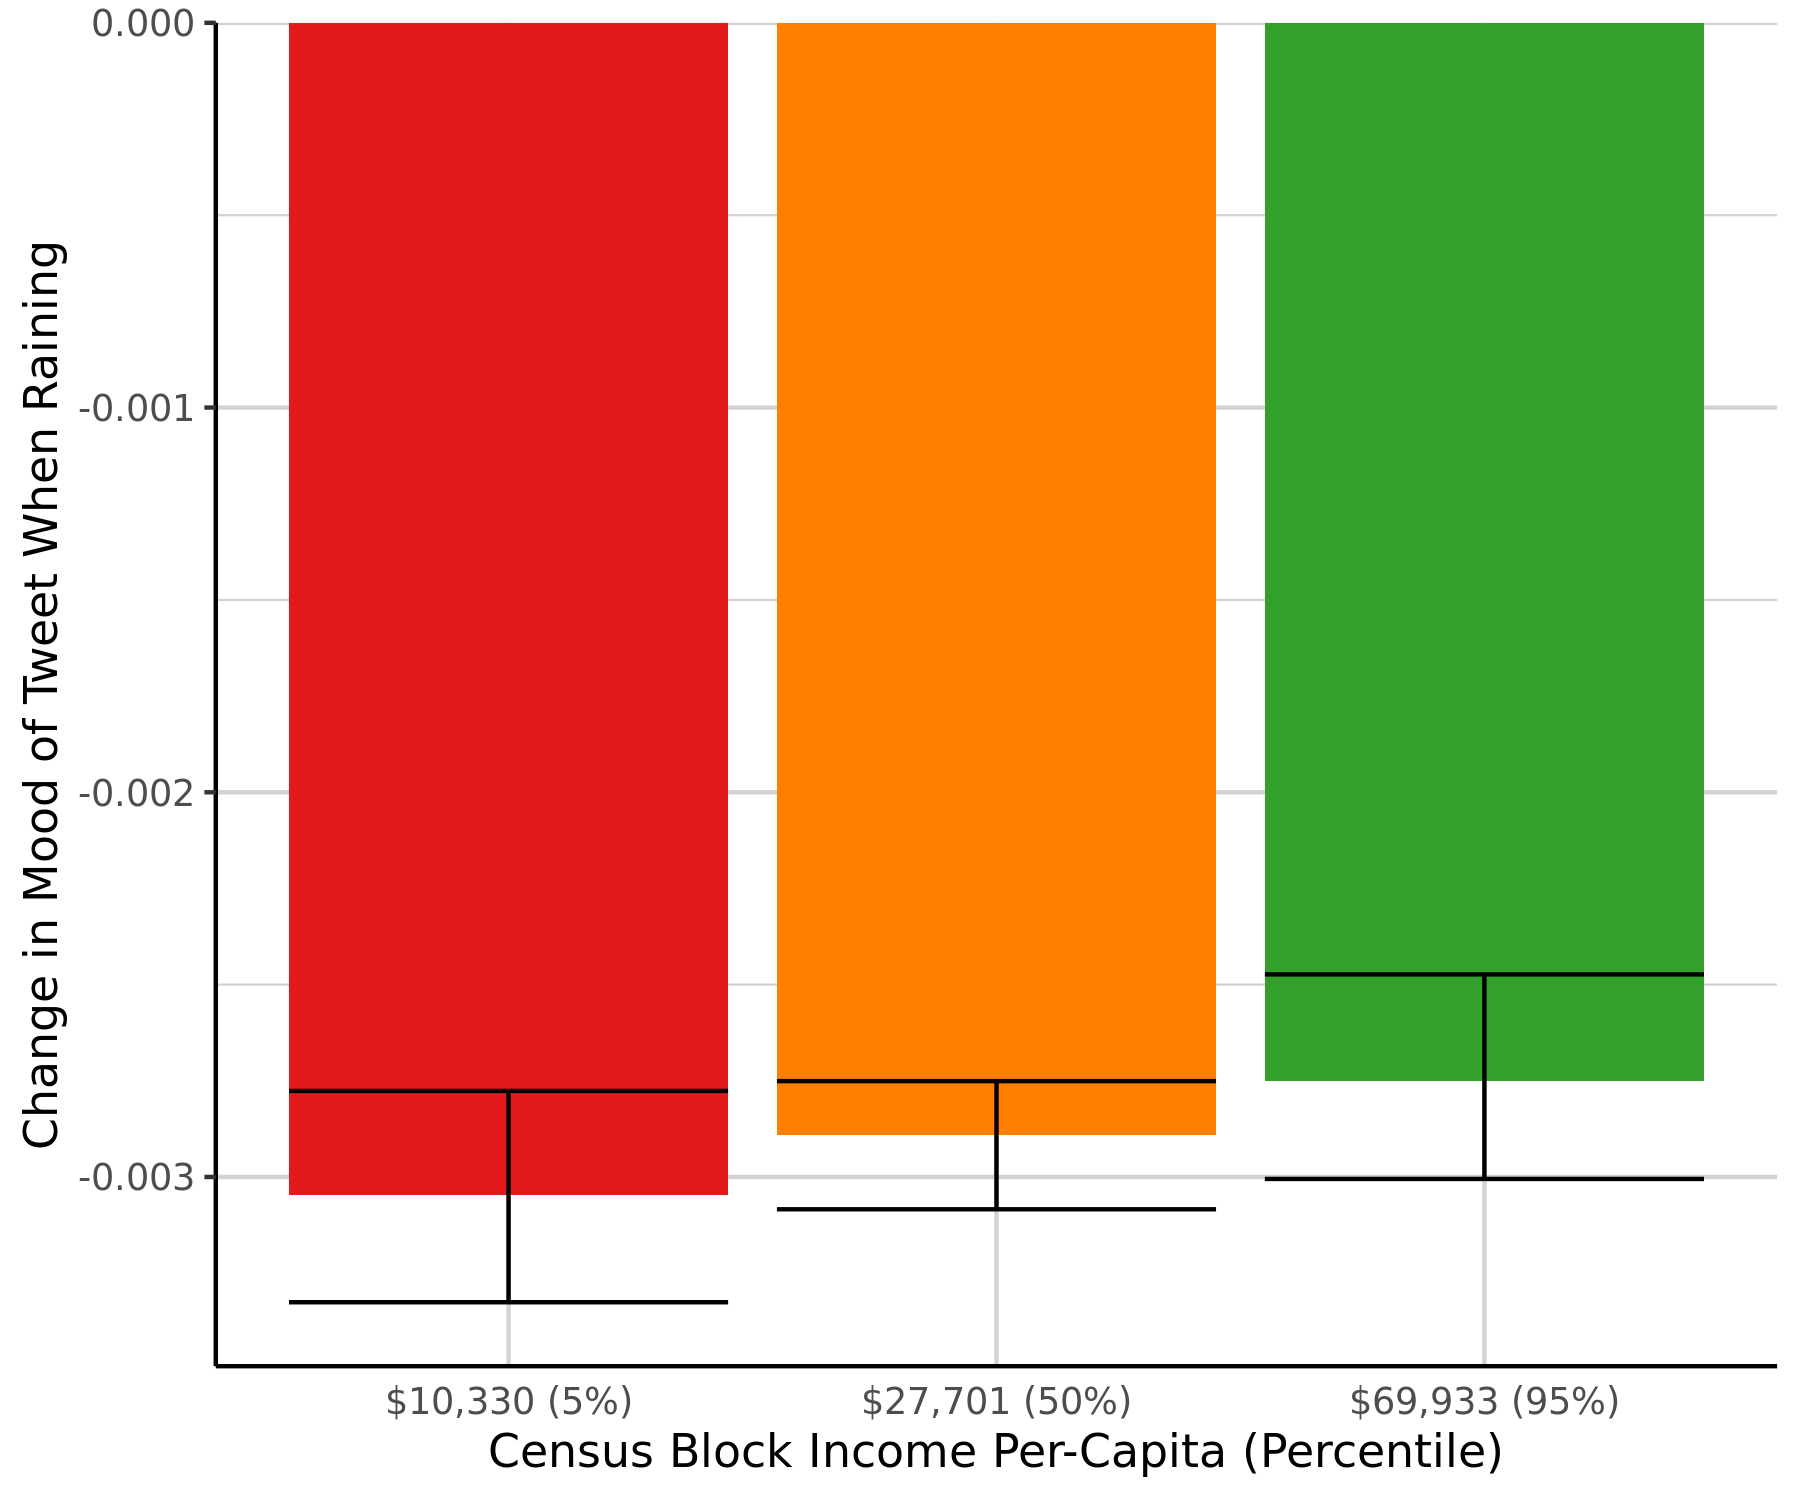
\includegraphics[width=0.6\linewidth]{../res/raining-income.png}
  \caption{Effect of rain on sentiment and moderated by income.}
  \label{fig:timeseries}
\end{figure}

\begin{figure}[H]
  \centering
  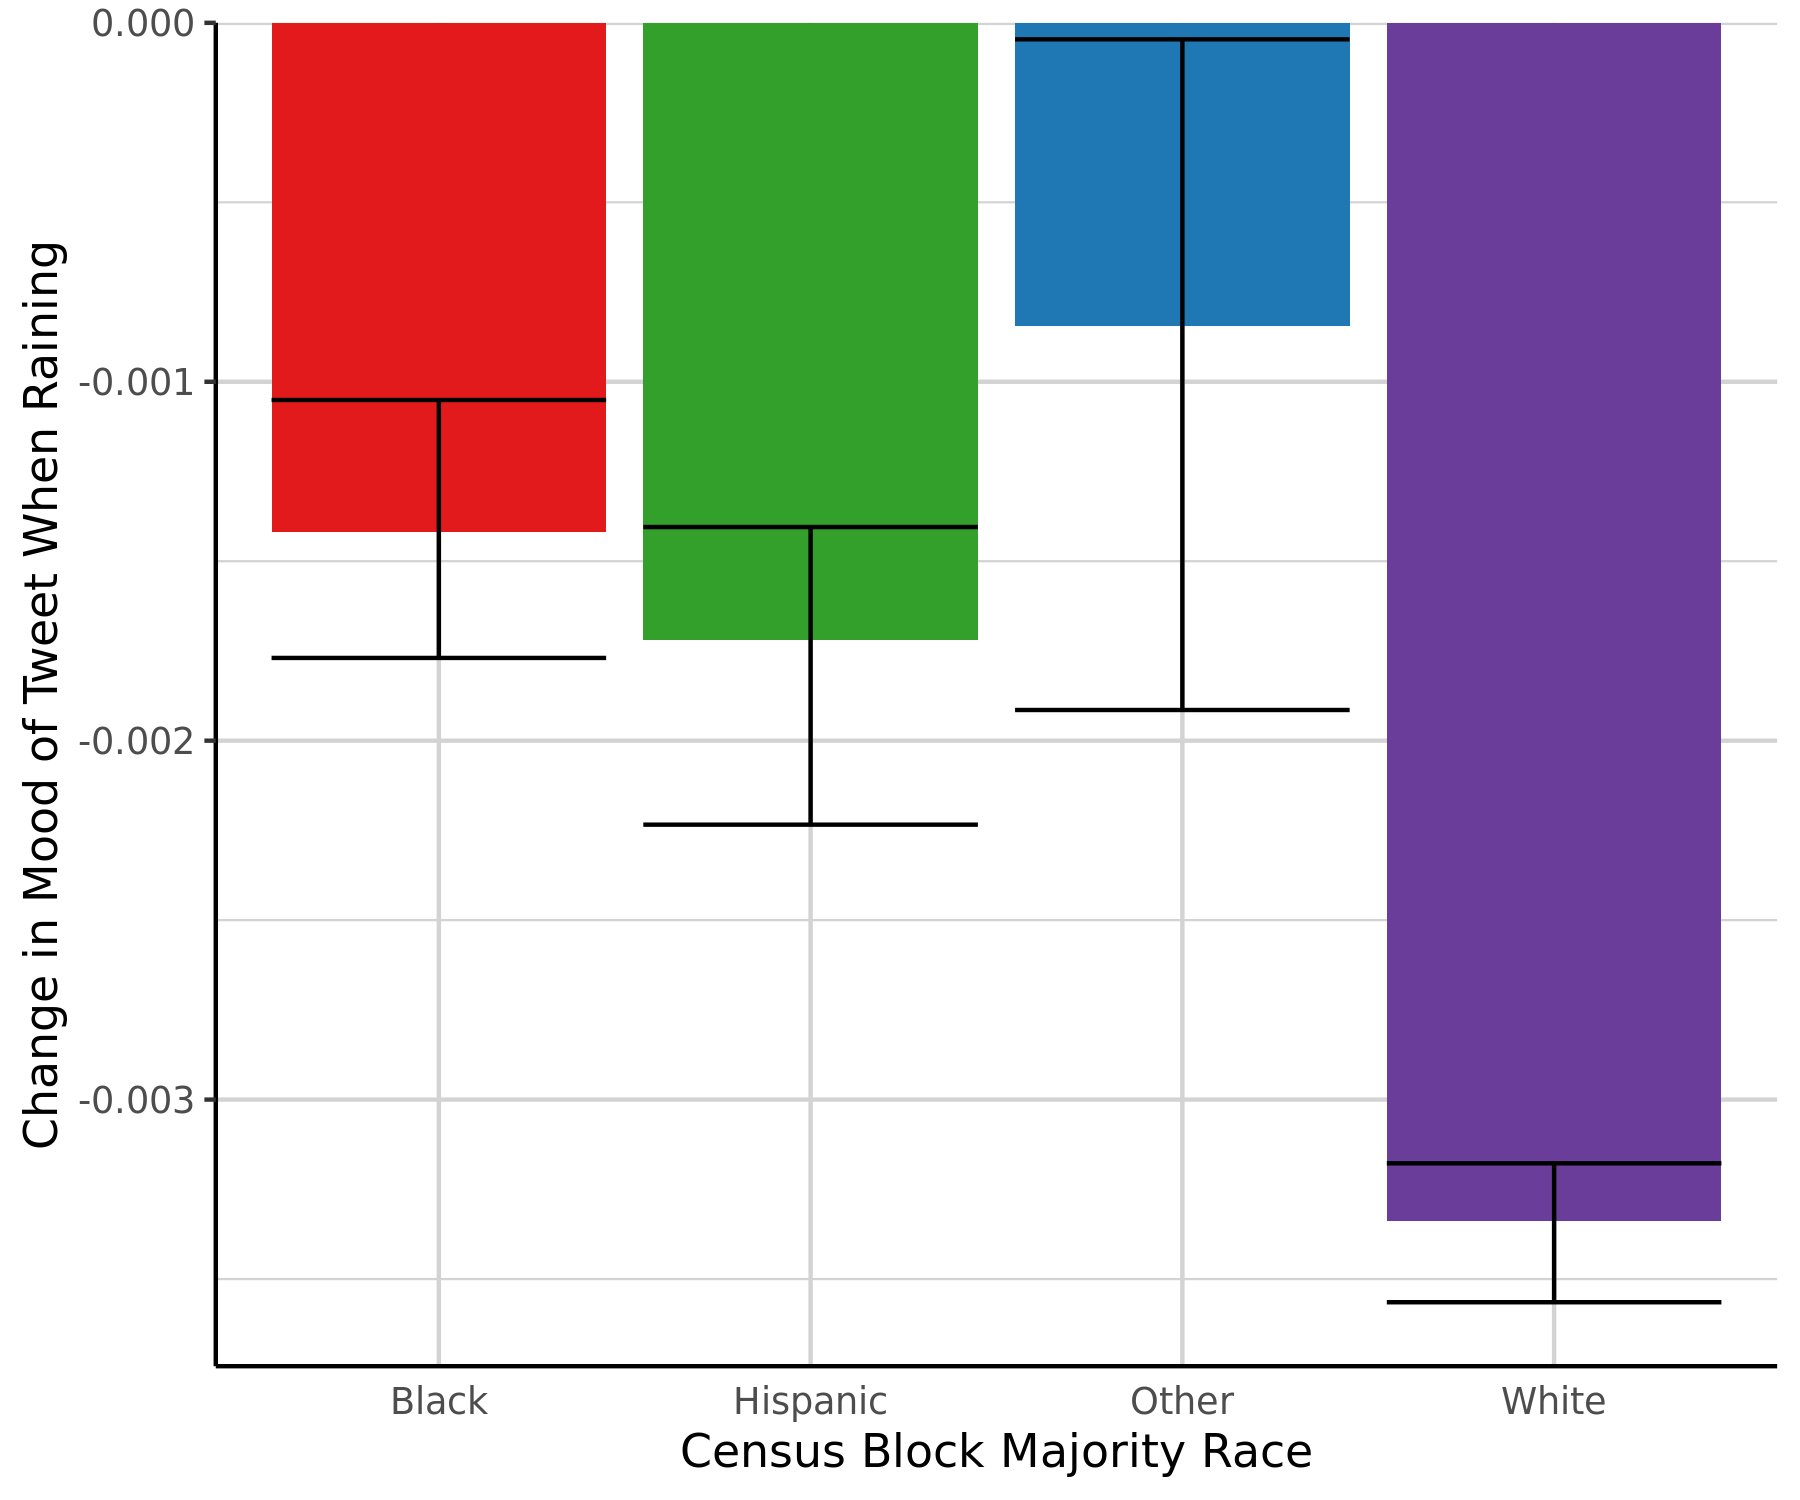
\includegraphics[width=0.6\linewidth]{../res/raining-race_q.png}
  \caption{Effect of rain on sentiment and moderated by race.}
  \label{fig:timeseries}
\end{figure}


\begin{figure}[H]
  \centering
  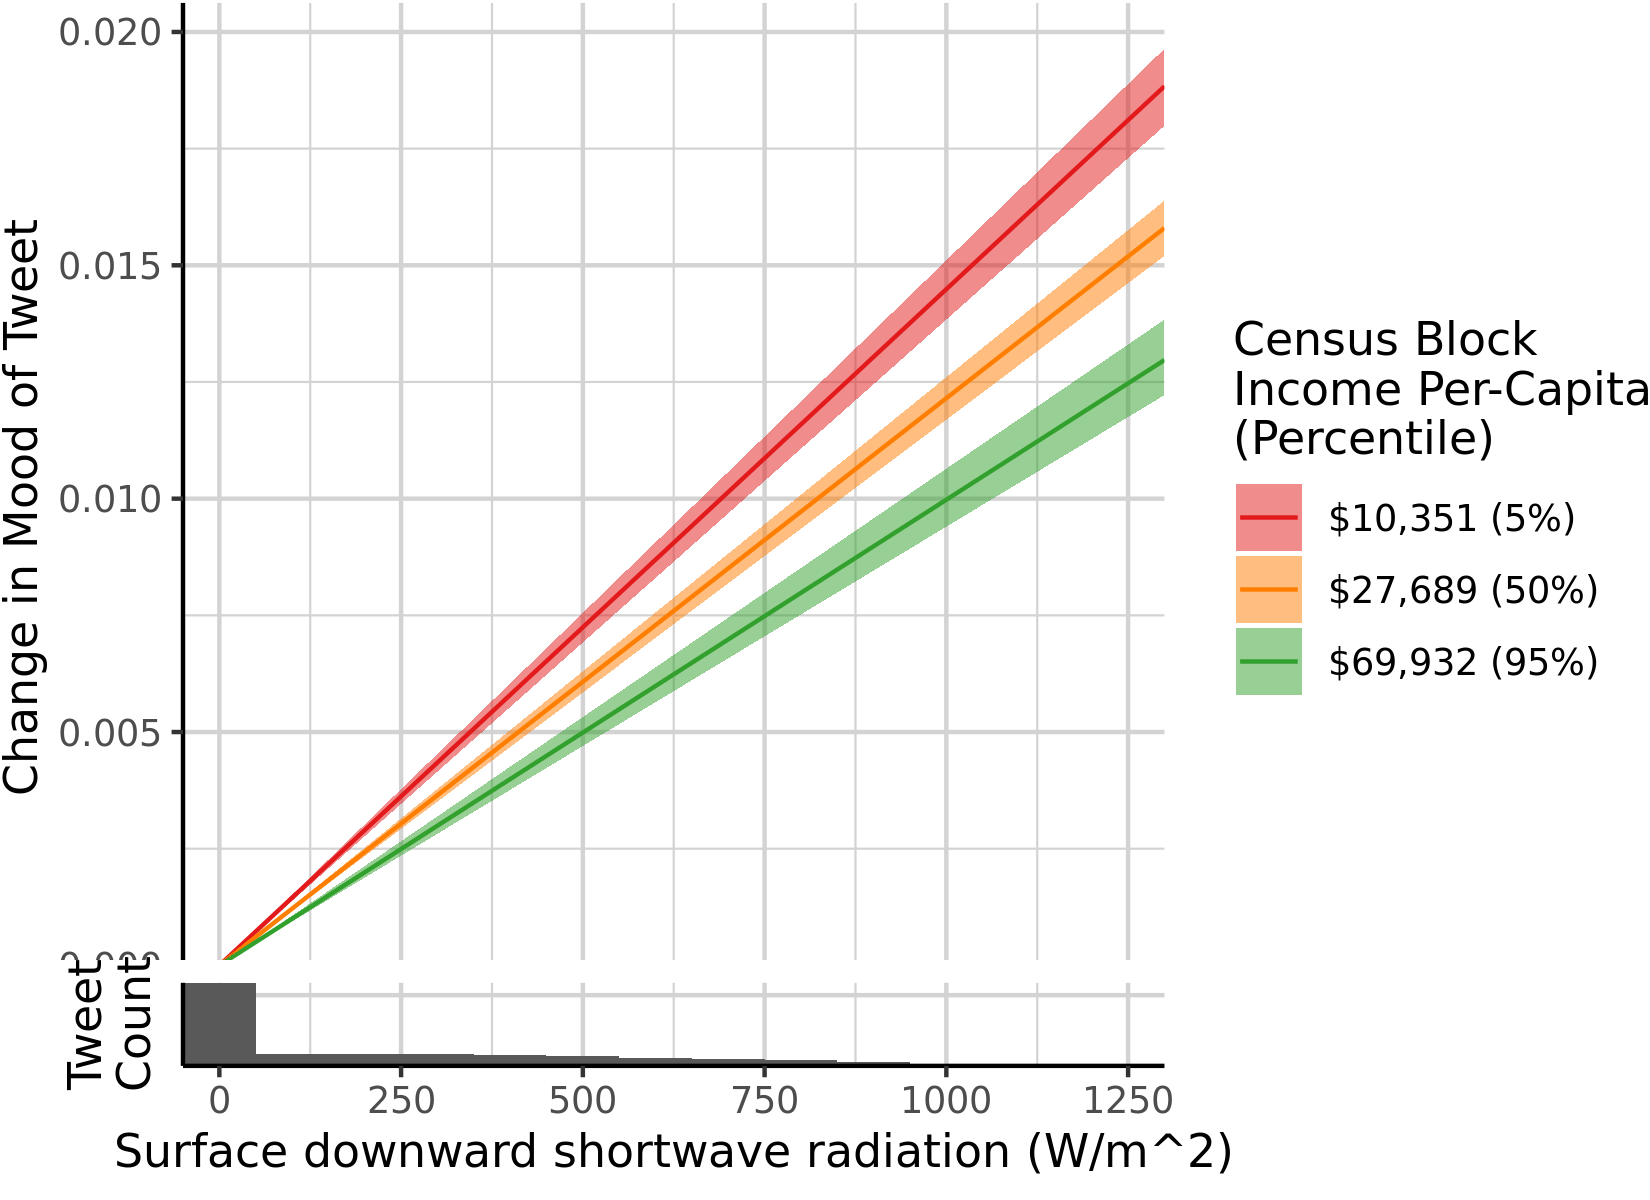
\includegraphics[width=0.6\linewidth]{../res/srad-income.png}
  \caption{Effect of sunshine on sentiment and moderated by income.}
  \label{fig:timeseries}
\end{figure}

\begin{figure}[H]
  \centering
  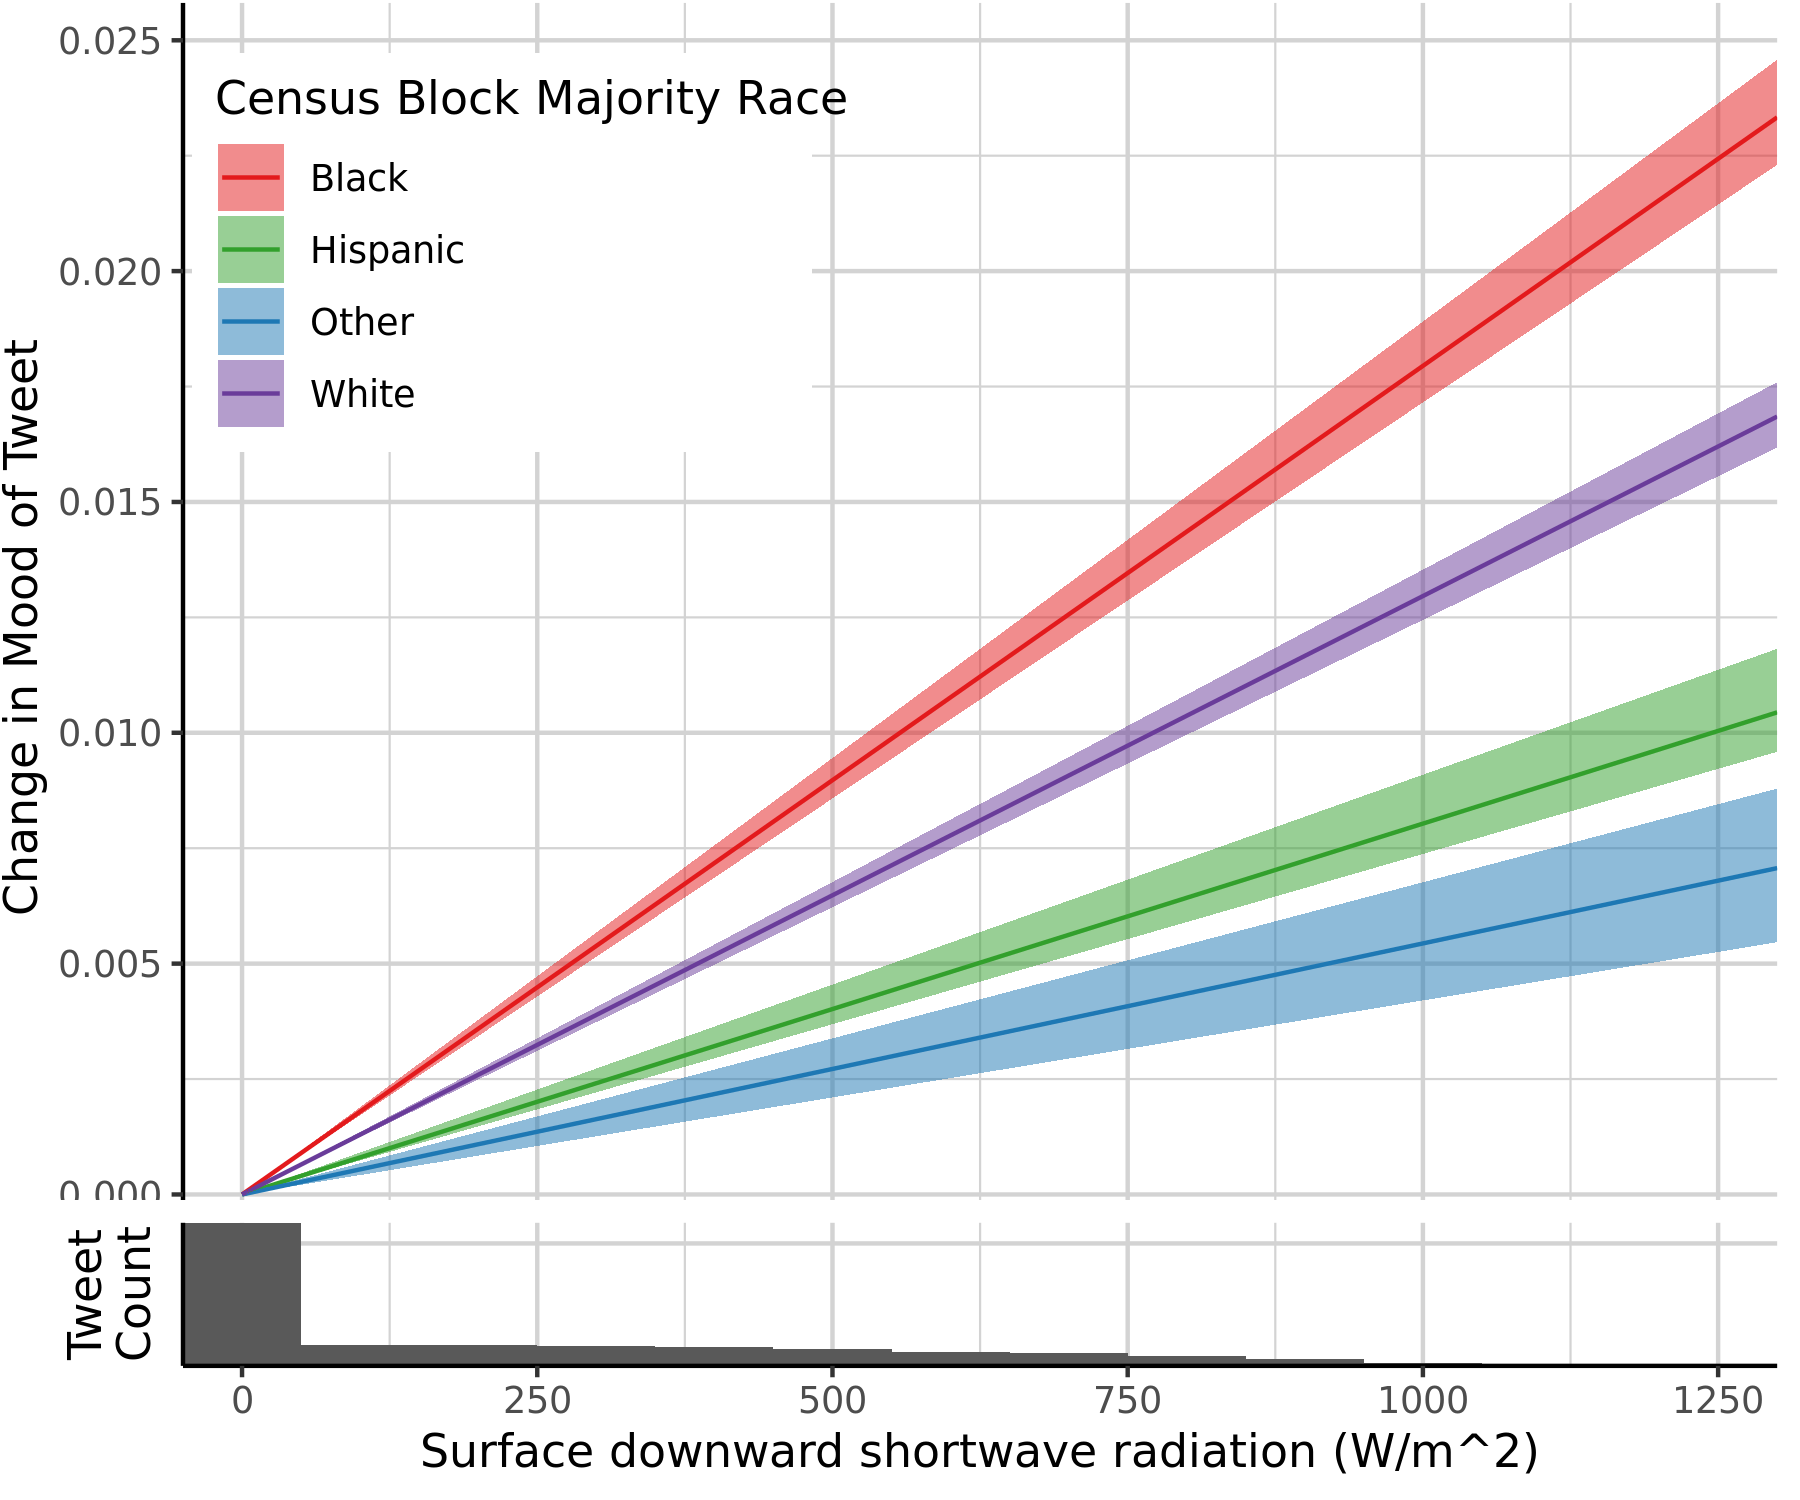
\includegraphics[width=0.6\linewidth]{../res/srad-race_q.png}
  \caption{Effect of sunshine on sentiment and moderated by race.}
  \label{fig:timeseries}
\end{figure}

\section{Combined Effects of Race and Income}

In addition to our models exploring how income and race moderate the effect of heat on sentiment, we fit an additional model with an interaction terms for both race and income.  Due to the complexity of a model with spline terms interacting with two different variables, using a categorical variable for race would have yielded a model matrix too large for the largest cloud virtual machine availale to us.  Thus, we used a continuous metric for both income as well as race (percent non-white/minority).

To examine how income and racial groups together moderate the effect of heat on sentiment, we extend our main model to the following form:

\begin{equation}
    y = \begin{tabular}{l}
    \beta_0 + f_t(t) + f_{m_{i}t}(m_{i} t) + f_{m_{r}t}(m_{r} t) + 
    \beta_p p + \beta_{m_{r} p} m_{r} p + 
    \beta_{m_{i} p} m_{i} p + \beta_{m_{i} m_{r} p} m_{i} m_{r} p + 
    \\
    \beta_s s + \beta_{m_{i} s} m_{i} s + 
    \beta_{m_{r} s} m_{r} s + \beta_{m_{i} m_{r} s} m_{i} m_{r} s + 
    \Phi + \epsilon
    \end{tabular}
    \label{mod:2}
\end{equation}

Identically to the model in the main body of the paper, $y$ is the sentiment of a tweet, $t$ is the wet bulb globe temperature at the hour of the tweet, $p$ is a binary variable indicating whether it rained at the hour of the tweet, $s$ is the income shortwave radiation, or sunshine, in $W/m^2$, at the hour of the tweet, $\Phi$ is the spatio-temporal fixed effects, $\epsilon$ is the normally-distributed errors, and $f_t$ represented the segmented regression for $t$, with knots at -10\textdegree, 0\textdegree, 5\textdegree, 10\textdegree, 15\textdegree, 20\textdegree, and 25\textdegree C WBGT.  We estimate the 95\% confidence interval of our models using 80-fold bootstrapping.  

In this new model, $m_{i}$ is the log-transformed average income in the census block where the tweet originated, while $m_{r}$ is the racial composition of the census block, in terms of the percent of the population that was a minority.

\begin{figure}[H]
  \centering
  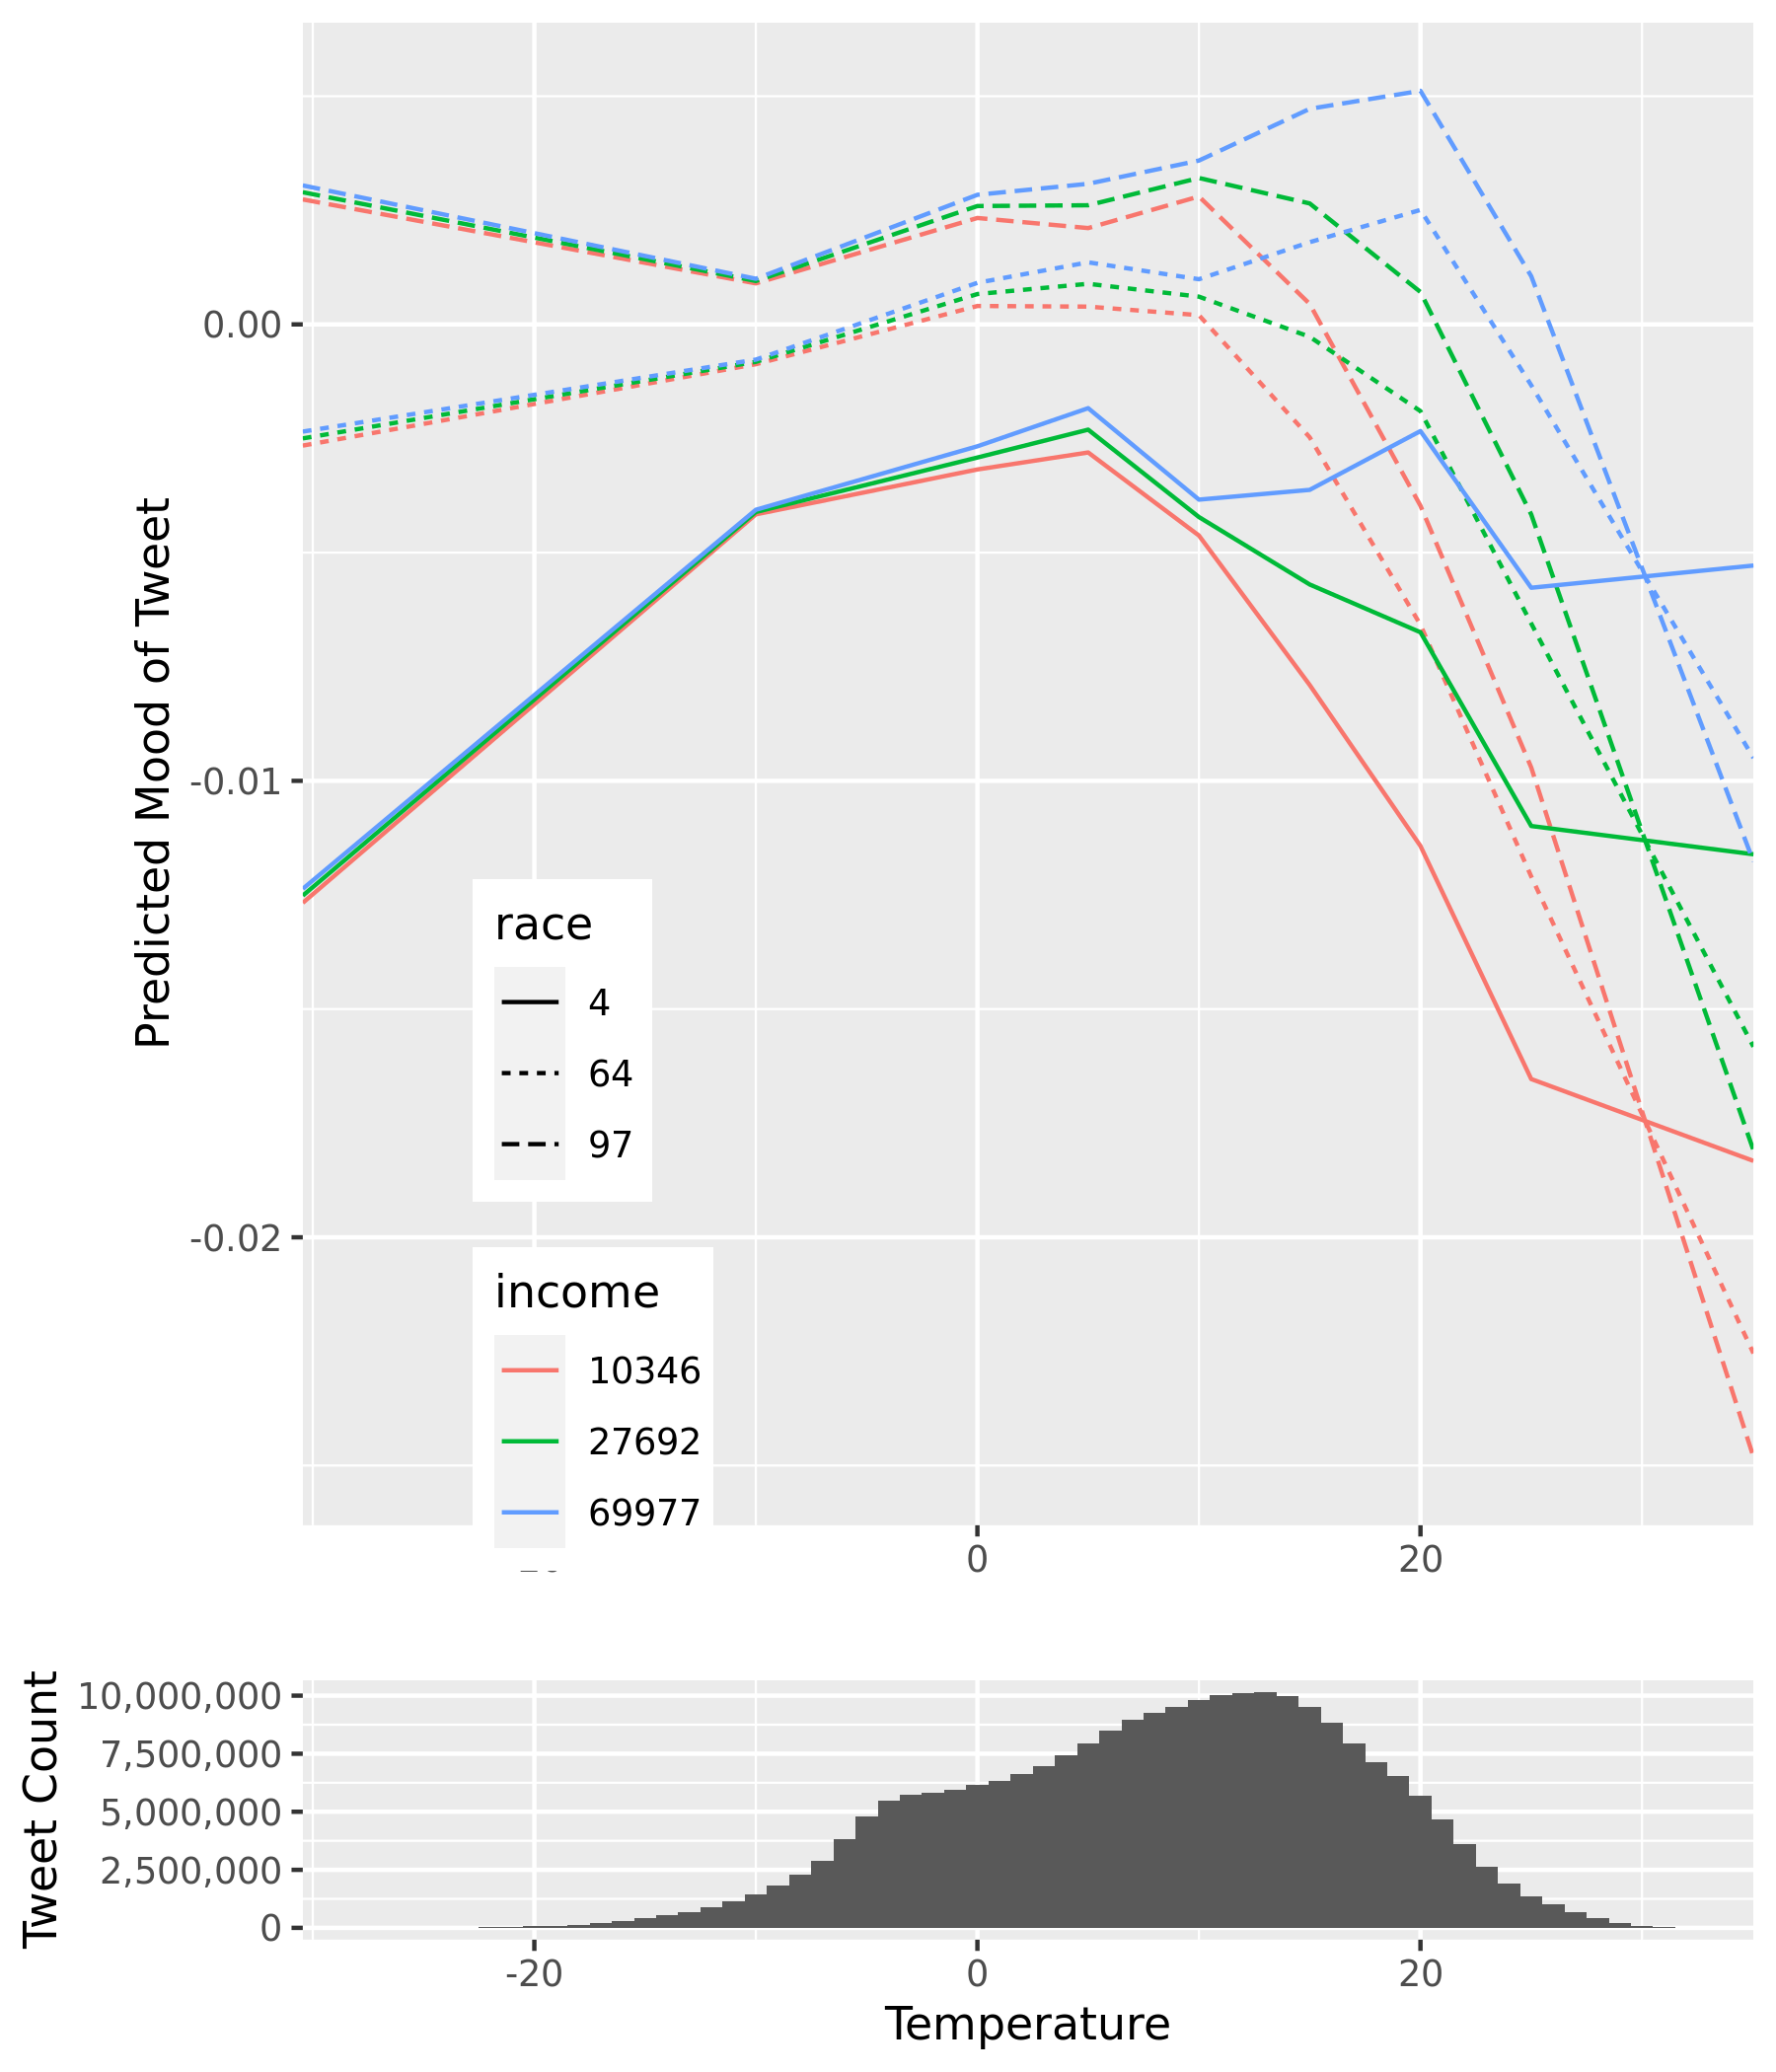
\includegraphics[width=0.6\linewidth]{../res/wbgt-income-race.png}
  \caption{Effect of temperature on sentiment and moderated by both race and income.}
  \label{fig:timeseries}
\end{figure}

\section{Weather Terms}
We excluded tweets that contained the following weather-related terms: aerovane, air, airstream, altocumulus, altostratus, anemometer, anemometers, anticyclone, anticyclones, arctic, arid, aridity, atmosphere, atmospheric, autumn, autumnal, balmy, baroclinic, barometer, barometers, barometric, blizzard, blizzards, blustering, blustery, blustery, breeze, breezes, breezy, brisk, calm, celsius, chill, chilled, chillier, chilliest, chilly, chinook, cirrocumulus, cirrostratus, cirrus, climate, climates, cloud, cloudburst, cloudbursts, cloudier, cloudiest, clouds, cloudy, cold, colder, coldest, condensation, contrail, contrails, cool, cooled, cooling, cools, cumulonimbus, cumulus, cyclone, cyclones, damp, damp, damper, damper, dampest, dampest, degree, degrees, deluge, dew, dews, dewy, doppler, downburst, downbursts, downdraft, downdrafts, downpour, downpours, dried, drier, dries, driest, drizzle, drizzled, drizzles, drizzly, drought, droughts, dry, dryline, fall, farenheit, flood, flooded, flooding, floods, flurries, flurry, fog, fogbow, fogbows, fogged, fogging, foggy, fogs, forecast, forecasted, forecasting, forecasts, freeze, freezes, freezing, frigid, frost, frostier, frostiest, frosts, frosty, froze, frozen, gale, gales, galoshes, gust, gusting, gusts, gusty, haboob, haboobs, hail, hailed, hailing, hails, haze, hazes, hazy, heat, heated, heating, heats, hoarfrost, hot, hotter, hottest, humid, humidity, hurricane, hurricanes, ice, iced, ices, icing, icy, inclement, landspout, landspouts, lightning, lightnings, macroburst, macrobursts, maelstrom, mercury, meteorologic, meteorologist, meteorologists, meteorology, microburst, microbursts, microclimate, microclimates, millibar, millibars, mist, misted, mists, misty, moist, moisture, monsoon, monsoons, mugginess, muggy, nexrad, nippy, NOAA, nor,’easter, nor,’easters, noreaster, noreasters, overcast, ozone, parched, parching, pollen, precipitate, precipitated, precipitates, precipitating, precipitation, psychrometer, radar, rain, rainboots, rainbow, rainbows, raincoat, raincoats, rained, rainfall, rainier, rainiest, raining, rains, rainy, sandstorm, sandstorms, scorcher, scorching, searing, shower, showering, showers, skiff, sleet, slicker, slickers, slush, slushy, smog, smoggier, smoggiest, smoggy, snow, snowed, snowier, snowiest, snowing, snowmageddon, snowpocalypse, snows, snowy, spring, sprinkle, sprinkles, sprinkling, squall, squalls, squally, storm, stormed, stormier, stormiest, storming, storms, stormy, stratocumulus, stratus, subtropical, summer, summery, sun, sunnier, sunniest, sunny, temperate, temperature, tempest, thaw, thawed, thawing, thaws, thermometer, thunder, thundered, thundering, thunders, thunderstorm, thunderstorms, tornadic, tornado, tornadoes, tropical, troposphere, tsunami, turbulent, twister, twisters, typhoon, typhoons, umbrella, umbrellas, vane, warm, warmed, warming, warms, warmth, waterspout, waterspouts, weather, wet, wetter, wettest, wind, windchill, windchills, windier, windiest, windspeed, windy, winter, wintery, and wintry.


\printbibliography

\end{document}
